\chapter{Conclusion}
\label{chap:conclusion}

This dissertation presents a motion planning approach suited for
multi-step manipulations tasks.
Key to the approach are the complementary ideas of \emph{lazy}
and \emph{utility-guided} search,
which we integrated into the LEMUR motion planning algorithm.
This approach has shown promising results on manipulation tasks
when compared with state-of-the-art
search-based and sampling-based anytime planners.
This concluding chapter begins by summarizing the dissertation
and the individual algorithmic contributions
in Section~\ref{sec:conclusion:summary}.
This is followed by a discussion in Section~\ref{sec:conclusion:future}
of a few promising avenues for future research
which build on our results,
as well as some lessons learned
in Section~\ref{sec:conclusion:lessons-learned}.
Finally, we offer some concluding remarks
in Section~\ref{sec:conclusion:remarks}.


\section{Summary and Contributions}
\label{sec:conclusion:summary}

This dissertation focuses on motion planning problems
which arise in autonomous manipulation tasks.
Such tasks induce continuous, high dimensional robot configuration
spaces
in which path validity checking is particularly expensive
due to complex robot kinematics and workspace geometry.
Furthermore,
there is an inherent cost tradeoff between
planning a motion and subsequently executing it.
For manipulation tasks in human-scale environments in particular,
whether measured in time or energy,
the cost of planning (principally path validity checking)
is comparable to the cost of execution.
Therefore,
reasoning over both sources of cost -- and their tradeoff --
is paramount.

To address these challenging motion planning problems,
this dissertation proposes a collection of algorithms
(Figure~\ref{fig:conclusion:outline})
which work in concert to minimize both planning and execution cost.
We first motivate our focus on roadmap methods for motion
planning,
and then consider two central questions concerning the search
over those roadmaps:
(a) how should we conduct the optimization,
and (b) what objective should we optimize?

\begin{figure}[t]
   \centering
   \includegraphics{build/outline}
   \caption{Outline of the algorithms developed in this dissertation.
      LEMUR is solves a continuous motion planning problem via
      discretization as a series of progressively densified roadmaps
      (Chapter~\ref{chap:roadmaps}).
      Since the shortest path problem over the resulting graph
      in characterized by edge costs which are expensive to evaluate,
      we exploit lazy search and edge selectors
      (Chapter~\ref{chap:lazysp}) to minimize planning effort.
      We also develop a novel incremental bidirectional search
      algorithm (Chapter~\ref{chap:ibid}) to accommodate the resulting
      dynamic pathfinding problem.
      LEMUR conducts its search guided by a utility function
      (Chapter~\ref{chap:utility}) which can employ distinct
      domain-specific planning and execution cost heuristics.
      In multi-step manipulation tasks,
      one such cost model is derived from the family motion planning
      problem (Chapter~\ref{chap:family}),
      which leads to planner invocations which minimize combined
      planning and execution cost.
      }
   \label{fig:conclusion:outline}
\end{figure}

\subsection{Motion Planning via Roadmaps}

In Chapter~\ref{chap:roadmaps},
we outlined the motion planning problem,
as well as a selection of algorithms designed to solve it.
A wide variety of such algorithms exist,
including optimization-based, search-based, and sampling-based
planners.
We motivate our focus on sampling-based roadmap planners
based on the following advantages:
\begin{itemize}
\item Roadmap methods are well-studied and possess favorable
   theoretical properties such as asymptotic optimality.
\item It is straightforward to incrementally densify the
   discretization by adding new samples to the roadmap.
\item The cost of constructing a roadmap which is
   insensitive to the distribution of obstacles can be amortized
   across all planning queries
   (e.g. loaded from disk and persisted in memory between queries).
\end{itemize}

The algorithms presented in this dissertation are agnostic to the
particular roadmap structure used for the discretization.
Our experiments were conducted over roadmaps generated
via Halton sequences,
with edges between vertices within a connection radius
determined by the critical value $\gamma^*_{\mathcal{C}}$.
For example, the LEMUR motion planner
(Algorithm~\ref{alg:lemur} in Chapter~\ref{chap:utility})
densifies its roadmap by introducing new batches of
vertices and edges;
in our experiments,
we reduce the connection radius as recommended in
\citep{janson2015deterministicsampling}.
We discuss future avenues for treating roadmaps
in Section~\ref{subsec:conclusion:future-roadmaps}.

\subsection{How to Optimize?}
Committing to a particular discretization (e.g. roadmaps)
reduces the continuous motion planning problem
to a discrete graph pathfinding problem.
The first central question considered in this dissertation, then,
is how a motion planning objective should be optimized over
such a roadmap graph.

\paragraph{Lazy Pathfinding.}
Pathfinding for motion planning problems is distinguished from other
shortest-path applications because
the primary component in its edge objective
depends on its \emph{validity},
which expensive to determine for articulated robots.
This motivates lazy pathfinding approaches,
which decouple the search for candidate solutions
from the process of evaluating each solution for its cost.

The first contribution of this dissertation is a study of
the LazySP algorithm outlined in Chapter~\ref{chap:lazysp},
\marginnote{Contribution: The LazySP algorithm,
which exploits an edge selector to find paths while
minimizing the number of necessary edge weight evaluations.}
which allows for this edge evaluation to be specified arbitrarily
by way of an \emph{edge selector} function.
We show that simple selectors are equivalent to the existing
Weighted A* and Lazy Weighted A* pathfinding algorithms,
and we also consider the efficacy of bidirectional
and bisection selectors.

We then introduce novel selectors based on path distributions,
which focus evaluations towards edges which most likely lie on
a shortest path.
One such path distribution selector is based on the partition
function over paths on a graph.
\marginnote{Contribution: an incremental method to maintain
the partition function over paths under changing edge weights.}
We develop an incremental method for 
We show that these selectors can lead to fewer expected edge
evaluations than their simple alternatives over a set of example
problems.
We also motivate why the alternating strategy serves as
a simple proxy for the more complex path distribution selectors
for common cases where no a priori knowledge of the obstacle
distribution exists.

We note that lazy planning over roadmaps accomplishes
the same evaluation focusing behavior exhibited by
informed sampling-based motion planners
\citep{gammell2014informedrrtstar, gammell2015bitstar}.
\cdnote{Add informed FMT* cite.}
LazySP naturally focuses evaluations only to areas which might improve
path cost of the particular query under consideration,
but due to the edge selector is not constrained to evaluate edges
only in cost-to-come order.

\paragraph{Dynamic Pathfinding.}
Conducting our roadmap search over candidate paths via lazy
pathfinding
induces an underlying inner dynamic shortest path problem.
This arises because the decoupled nature of lazy search
is indistinguishable from a search over an unknown or changing objective.
Each iteration of our lazy search constitutes a new dynamic planning
episode --
after our edge selector nominates particular edges of our roadmap
for evaluation and their true costs are determined,
the inner search must accommodate these changes in order to produce
new candidate paths on subsequent iterations.

Existing incremental algorithms for dynamic pathfinding problems,
such as Lifelong Planning A* \citep{koenig2004lpastar},
make use of heuristic potential functions to reduce the subset of
the graph that must be considered when solving each planning episode.
During a lazy search,
the strength of this heuristic depends on
the relationship between the true and estimated edge weights
($w$ and $w_{\ms{est}}$ in LazySP, respectively)
-- and in many cases, a strong lower bound on $w$,
and therefore a strong heuristic, may not exist.
This motivates our study of the dynamic problem
in Chapter~\ref{chap:ibid}.

A common approach to solving pathfinding problems in domains without
a strong heuristic is the notion of bidirectional search.
Unifying bidirectional and incremental methods presents a unique
challenge,
since the subtle bidirectional termination condition must be
posed in such a way that it remains applicable even under the
changing edge weights which arise in a dynamic problem.
This allows us to formulate the Incremental Bidirectional Dijkstra's
(IBiD) algorithm,
\marginnote{Contribution: the IBiD algorithm,
an incremental and bidirectional shortest path algorithm
for dynamic graphs.}
which generalizes the bidirectional Dijkstra's algorithm
\citep{goldberg2005spexternalmemory}
in the same way that the DynamicSWSF-FP algorithm
\citep{ramalingam1996dynamicswsffp} generalizes the original
Dijkstra's algorithm \citep{dijkstra1959anote}.
We also show how this algorithm can be adapted in the presence of
heuristic potential functions.
This algorithm shows promising results both on road network routing
problems (Chapter~\ref{chap:ibid})
as well as inflated lazy search problems from motion planning.

\subsection{What to Optimize?}
Our treatment of lazy roadmap search deliberatively leaves open
the question of what objective should be optimized.
The approach is applicable to any pathfinding domain in which
the edge weight function $w$ is expensive to evaluate,
and where an inexpensive estimate $w_{\ms{est}}$ may be available.
In the case of motion planning for articulated robots,
where planning and execution cost are both important,
how should we instantiate these functions?

\paragraph{Search over Candidate Utility.}
In Chapter~\ref{chap:utility},
we introduce the notion of \emph{utility},
and argue that it is the correct form of the objective in order
to capture the tradeoff between planning and execution costs.
Our conception of utility borrows heavily from the BUGSY algorithm
\citep{burns2013bugsy} for conventional graph search.
The key insight is that marrying utility with lazy search
allows for the incorporation of planning cost estimators over
concrete candidate paths -- and not just over frontier vertices.
This enables many domain-specific planning heuristics to be
represented naturally.

We next show that by committing to
(a) a utility function that is linear in planning and execution cost,
and (b) estimators that are additive over path edges,
we can represent our utility optimization as a lazy shortest path
problem.
Mediated by the tradeoff parameter $\lambda_p$,
the LEMUR algorithm
\marginnote{Contribution: the LEMUR motion planning algorithm
which conducts a lazy search guided by path utility over a set of
sequence of densified roadmaps.}
conducts this optimization
over a sequence of progressively densified roadmaps.

We examine a set of manipulation planning tasks using three
robot platforms,
and conduct experiments using a planning cost heuristic which
captures the remaining collision checks on each candidate path.
We show that LEMUR exhibits favorable performance
when compared against a set of anytime planners
such as RRT-Connect, BIT*, and Lazy ARA*.

\paragraph{Utility Estimates in Manipulation Planning.}
Importantly,
the utility-based objective described in Chapter~\ref{chap:utility}
allows arbitrary domain-specific planning cost estimates
to be leveraged.
Chapter~\ref{chap:family} explores intelligent heuristics
in manipulation tasks by formulating such multi-step tasks as
a \emph{family motion planning problem}.
\marginnote{Contribution:
the family motion planning problem
a formulation of manipulation planning that yields a natural
planning cost estimate for utility-guided motion planners.}
We show this representation,
in which multi-step tasks are given over a family of related
C-space subsets,
allows for a planning cost heuristic
which naturally incentivizes a utility-based planner (such as LEMUR)
to reuse planning computation from prior queries.


\section{Future Directions}
\label{sec:conclusion:future}

Treating motion planning as a lazy search over roadmaps
prompts an array of promising directions for further work.
Improvements in roadmap discretization,
focusing of edge evaluations,
better inner search algorithms,
more expressive domain-specific planning and execution cost
heuristics,
and probabilistic optimization techniques might all improve performance
over a wide array of planning domains.
In this section,
we survey a few such promising directions that arise from our
approach.

%The remainder of this chapter discusses both the implications
%and limitations of the presented approach,
%as well as possible directions for future work.
%In this chapter,
%we discuss opportunities to extend our approach to achieve even
%better performance,
%examine options to better integrate motion planning into a
%task planning system,
%and expound on other promising future directions.

\subsection{Improved Roadmaps}
\label{subsec:conclusion:future-roadmaps}

One of the fundamental questions in any motion planning approach
is how should the continuous problem be approximated in order
to search for a solution.
The approach to motion planning presented in this dissertation
relies fundamentally on the roadmap discretization method.
The approach can therefore benefit from any technique which improves
the efficacy of this discretization.

\paragraph{Better Connection Heuristics.}
Roadmap methods rely on a connection rule to determine whether
two vertices representing configurations in the C-space
should be connected with an edge
-- the existence of such an edge implies that the local planner
has high likelihood of successfully finding a valid path between them.
To this end,
most approaches make use of arbitrary thresholds of
simple distance functions over $\mathcal{C}$ as their decision rules.
In our experiments, for example,
we used a simple Euclidean distance rule.

However, for articulated robots
(and especially for recurring tasks in similar environments),
it is easy to conceive of more intelligent connection rules.
For example, consider a na\"{\i}ve execution cost model in which
obstacles are distributed uniformly in the robot's workspace.
In this case,
the likelihood of collision over some edge length
depends on the configuration of the arm itself
-- configurations in which the Jacobian matrix is large
(where changes in the location of robot geometry are large
with respect to changes in configuration)
entail higher collision probability.
In the case of recurring motion planning queries for the same
robot geometry,
it would seem beneficial to pre-compute a roadmap structure
in which the edge connection rule depends on some similar measure
of the robot's configuration.

%\paragraph{Efficient Densification.}
%The LEMUR motion planner conducts its search over a series of
%progressively densified roadmaps.
%We currently precompute these roadmaps up to a particular level
%of discretization.
%Smarter sequences that are easy to densify.
%Fractal patterns?
%Not lattices.
%Parallelization.
%Recent RSS results?

\subsection{Adaptive Roadmap Densification via an Infinite Roadmap Stack}
\label{subsec:conclusion:infinite-stack}

\label{sec:discussion:disc}
The LEMUR planner effectively conducts its search over a sequence of
progressively densified roadmaps
(Figure~\ref{fig:discussion:roadmap-stack}).
The results presented in this thesis have used Halton sequences
as discussed in Chapter~\ref{chap:roadmaps}
for their preferable dispersion properties,
and form a roadmap graph using an $r$-disk connection rule.
As discussed in \citep{janson2015deterministicsampling},
the shortest path on such a sequence of roadmaps
possesses asymptotic optimality if the connection radius is adjusted
appropriately.

\begin{figure}
   \centering
   \includegraphics{build/roadmap-stack}
   \caption{A stack of progressively densified roadmaps
      over a given free configuration space $\mathcal{C}$.}
   \label{fig:discussion:roadmap-stack}
\end{figure}

\paragraph{Hard batching.}
Like many existing roadmap-based algorithms
\citep{starek2015bfmtstar, gammell2015bitstar},
LEMUR implements a hard batching approach to densification --
a search is conducted fully over each batch of the roadmap
in $\mathcal{C}$
until a solution is found.
While the specification of LEMUR allows for this roadmap to be
implicitly constructed,
the current implementation constructs the entire batch before
proceeding with its search.
Once the search over that roadmap completes without a feasible path found,
the next batch of vertices and edges are added to the graph,
and the newly densified roadmap is searched.

Because the sequence of roadmaps that is searched is insensitive to
the distribution of obstacles,
the current implementation of LEMUR is able to pre-compute a sequence
of roadmaps up to a certain level of discretization,
and then load that roadmap structure into memory directly
instead of building it from scratch for each planning query.

There are two shortcomings that arise from this hard batching approach:

\begin{itemize}
\item \emph{Uniform Densification:}
   The fact that this roadmap is loaded uniformly across the space
   is certainly a limitation that will become restrictive
   in spaces of larger dimension.
\item \emph{Densification vs. Resolution Completeness:}
   The current LEMUR algorithm only moves to a denser roadmap
   once no finite paths are shown to be available on the present
   roadmap.
   This may not be desirable in large spaces --
   it may make sense to move to a denser roadmap in the vicinity of
   a short path before exploring all corners of the space.
\end{itemize}

There are a number of promising avenues for a solution
to the problems that arise from uniform densification..
Informed anytime algorithms
\citep{gammell2014informedrrtstar, gammell2015bitstar}
restrict densification once an initial path is found to a subset of
the full space that may contain better solutions.
This approach is not directly applicable
because LEMUR is not an anytime algorithm.

\paragraph{Adaptive Roadmap Densification.}
An alternative strategy is to adopt an adaptive densification approach
under which the search is conducted upon an infinite stack of
progressively densified roadmaps.

Consider the roadmap stack depicted
in Figure~\ref{fig:discussion:roadmap-stack-onramps}.
Here, as before,
each underlying roadmap is a superset of the one above it.
But now,
instead of progressively considering each layer individually
(using batching),
consider conducting a single search over the entire stack.
Note that the stack includes additional edges
(shown dotted in the figure)
connecting corresponding vertices in two adjacent layers;
using a road network analogy,
we call these edges ``offramp'' edges.
A proposed edge weighting scheme involves two components:
(a) an artificial inflation of edge weights by some factor
on each layer according to a schedule
(with edges on lower layers inflated more),
and (b) an artificial constant weight assigned to each offramp edge
between layers.

%Related to the idea of adaptive dimensionality
%\citep{gochevetal2011adaptivedim}
%(large portions of solutions can be low-dimensional).

\begin{marginfigure}
   \centering
   \includegraphics{build/roadmap-stack-onramps}
   \caption{A roadmap stack with ``offramp'' edges.}
   \label{fig:discussion:roadmap-stack-onramps}
\end{marginfigure}

Consider a search over this infinite stack $G$
between two start and destination
configurations corresponding to distinguished vertices on $G$,
and consider an optimal solution path with strong $\delta$-clearance.
If the roadmap layers satisfy the appropriate conditions
(e.g. connection radius
\citep{karaman2011samplingoptimal, janson2015deterministicsampling}),
and all roadmap edges have nonnegative weight,
and all ``offramp'' edges have some constant positive weight $\alpha$,
then we conjecture that there exists a shortest path $p$ through $G$
of finite length (which traverses a finite number of layers of $G$).
Furthermore,
we conjecture that the length of $p$ approaches the length of an
optimal path as $\alpha \rightarrow 0$.

We find this representation of the continuous problem compelling
because it naturally integrates the densification problem with
the search problem.
One can imagine a unidirectional or bidirectional search
effectively trading off between
exploring more widely on a particular layer
and descending to a denser layer in order to traverse a narrow passage.
Descending to a denser layer occurs naturally during the search,
and denser regions can be sampled on demand only in areas of the space
adjacent to obstacles blocking the path.
Furthermore,
the computational cost of such densification can be captured as
an additional planning cost component in the LEMUR algorithm,
\marginnote{Opportunity for a more accurate planning cost estimate:
adding a term for expected cost of a further roadmap densification.}
so it will commit to a denser layer only when the predicted path
savings outweigh the requisite planning cost.

\subsection{Improved Lazy and Dynamic Search}

The core of our approach is a lazy search over candidate paths,
which makes use of an inner dynamic shortest path problem
in order to select candidates at each iteration.
There are a number of potential avenues available for making this
search more efficient.

\paragraph{Intelligent Selection of Key Edges.}
In Chapter~\ref{chap:lazysp},
we presented novel edge selectors which maintain a distribution over
candidate paths
in order to focus edge evaluations towards edges which most likely
lie on a short path.
While this showed promising results across a range of problem instances,
maintaining this distribution can incur its own computational cost
(quadratic in the number of vertices in the case of the Partition
selector),
and therefore it can be intractable over large roadmap graphs.

The effect of these selectors is to automatically discover
and focus on the parts of the motion planning problem that are
most constrained.
It would be worthwhile to explore ways of more efficiently maintaining
such path distributions for larger graphs.
In the case of a bidirectional evaluation strategy
(such as the Alternate selector),
it may be beneficial to attempt to discover online which end
of the problem proves to be the most constrained.

It may also be instructive to investigate the ``oracle'' selector.
Consider that for any graph,
there exists some minimal set of edges which, if evaluated,
would probably demonstrate that the best remaining candidate is
correct.
Investigating the distribution of edges required for such a selector
for particular problem instances
may aid in designing new selectors.
It also serves as a useful benchmark against which to compare performance.

\paragraph{Exploring the Interaction between Lazy and Dynamic Search.}
Lazy search induces an inner dynamic shortest path problem,
as edge weights are updated and intermediate candidate paths are
required.
When LEMUR addresses a problem with $\lambda_p > 0$,
so that planning cost is to be considered in its utility objective,
it generally selects candidates that do not solely minimize execution cost
in favor of candidates that lower remaining planning cost.

Paradoxically,
as the $\lambda_p$ parameter is increased,
the underlying dynamic search problem becomes more difficult,
because its heuristic is no longer as strong.
(A consistent heuristic typically only exists for the component of
the edge weight function derived from the execution cost component.)
It would therefore be beneficial to investigate schemes whereby
the requirement for optimal shortest paths from the inner
dynamic search is relaxed.
For example,
consider a variant of the LazySP algorithm
in which the candidate path at each iteration only maximizes utility
up to a particular suboptimality bound. 
One suitable algorithm for this relaxed dynamic search problem
is Truncated Incremental Search \citep{aine2016truncatedincremental}.

\paragraph{Adjusting the Incremental Balancing Criterion.}
It is well-known \citep{pohl1969bidirectional}
that using the cardinality of each OPEN list as the decision rule
to balance expansion of the two sides of a conventional bidirectional
search generally outperforms using the distance (key) value itself.
Unfortunately,
it is not clear how to adapt this criterion to the incremental
search setting,
since the size of the queue of inconsistent vertices is no longer
indicative of the density of the graph on the two sides.
Can we dynamically adjust the distance balance criterion
so that the location of the interface between the two trees
(represented as the edge connection queue)
approximates this balanced cardinality criterion?

\paragraph{Modeling and Incorporating Search Cost.}
The LEMUR planning cost heuristic allows estimates of remaining
planning cost to be incorporated into the planner's utility function.
For our experiments in this dissertation,
this planning cost term included a measure of the expected
collision checking cost remaining.
However,
for larger or denser graphs,
the time to conduct the inner search may become important to model
as well.
\marginnote{Opportunity for a more accurate planning cost estimate:
adding a term for expected search cost.}
If such a model exists,
the planner could (for example) use it to determine
whether to proceed with a new search,
or whether to terminate immediately with the best path it has
found so far.

\subsection{Tighter Integration with Collision Validity Checking}

The basic motion planning problem described in Chapter~\ref{chap:roadmaps}
considers arbitrary configuration space obstacles.
When most sampling and search based motion planners test
candidate path segments for validity,
they treat validity checking
-- usually via a geometric collision checker --
as a ``black box'' operation.
Given a test configuration $q_{\ms{test}}$,
such a checker considers the environment
and the robot's kinematics,
and returns a boolean answer -- True or False.
Depending on the fidelity of the geometric model of the robot
and environment,
each check can entail tens, hundreds, or even thousands
of microseconds.
There are a number of opportunities for extending LEMUR in order
to better predict and account for the internal mechanisms of these
checkers.

Chapter~\ref{chap:family} explored one such opportunity --
decomposing the validity checks performed over multiple steps of
a manipulation task as a family motion planning problem.
Doing so allows a planning cost model to be formulated naturally
in terms of different subsets of C-space,
so that a utility-aware planner (such as LEMUR)
is incentivized to reuse partial validity information
from cached or previous similar planning episodes.
In this section,
we discuss other opportunities for characterizing and breaking
the black box collision checking abstraction.

\paragraph{Better Estimates of Expected Validity Checking Cost.}
The experiments in this dissertation relied on a simple model for
the planning cost required for each collision check.
First,
a single averaged duration per collision check was learned over an array
of problems for each robot platform.
Then, during the course of a planning query,
the remaining planning cost required for each candidate path
consisted simply of this duration summed across all remaining
configurations to be checked.
\marginnote{Opportunity for a more accurate planning cost estimate:
a model for the different planning cost required in different parts of the space.}

This simple model could be improved in at least two ways:
\begin{itemize}
\item First, the planning cost required for a collision check could
   be learned dynamically during a planning episode.
   The cost per check depends on the complexity of the workspace
   obstacles and the areas of the configuration space actually
   explored,
   and a planner which incorporates such learning could better adapt to
   particular planning queries and manage its search more accurately.
\item Second, the planning cost required for a collision check depends
   on the area of configuration space itself.
   For example,
   checks in wide open spaces tend to complete much more quickly than
   those near obstacle boundaries.
   A planning cost estimator could build and maintain a spatial model
   of this checking cost during the course of a planning episode,
   and adjust the predicted remaining planning costs for candidate
   paths as a result.
\end{itemize}

\begin{figure*}[t]
   \centering
   
   \subfloat[
      A motion planner testing simply for membership in
      $\mathcal{C}_{\mbox{\scriptsize free}}$
      treats a collision validity checker as a
      ``black box.''
      Internally,
      modern checkers first employ an inexpensive broad-phase check
      using a simple conservative representation
      to quickly identify non-colliding bodies before
      resorting to an expensive narrow-phase check.
   ]{%
      \includegraphics{build/broadphase-single}%
   }%
   \quad%
   \subfloat[
      A family motion planner can explicitly reason about the
      conservative nature of the broad-phase check.
      This allows it to defer many narrow phase checks
      (often indefinitely)
      and instead prefer paths that require fewer expensive checks.
   ]{%
      \includegraphics{build/broadphase-multi}%
   }
   
   \caption[][0.0in]{Collision validity checking is a commonly used
     indicator function.
     The family motion planning formulation allows an intelligent
     planner to reach inside the checker's ``black box''
     and reduce the number of costly narrow-phase checks.
     Resulting paths tend to be cheaper to compute and
     stay further from obstacles.}
   \label{fig:broad-phase}
\end{figure*}

\paragraph{Exploiting Multi-Phase Collision Checkers.}
Many geometric collision checkers build a multi-phase hierarchy,
both to quickly answer easy validity queries,
and to focus computation to areas where determining validity
requires checking at a finer resolution.
One of the most widely used approaches entails building
a simple conservative geometric approximation
(e.g. a bounding box),
and first checking that approximation for collision during an
initial ``broad-phase'' check.
Only geometry which fails this check is then subjected for
subsequent (and more expensive) ``narrow-phase'' checking.
See Figure~\ref{fig:broad-phase} for example of such a multi-phase
validity checker.

Most motion planners treat the validity checker as a binary
``black box,''
and do not explicitly reason about this underlying multi-phase process.
However,
it may be advantageous for the planner to be made aware of these
phases.
This allows the planner to effectively identify configurations for which
many (or all) geometric pairs are sufficiently far from collision
that the more expensive narrow-phase checks need not be applied.
In fact,
this structure can be represented simply as a family motion planning
problem.
Consider the two subsets of configuration space
$B \subseteq \mathcal{C}$ and $N \subseteq \mathcal{C}$
which satisfy the inexpensive broad-phase and expensive narrow-phase
checks, respectively.
It is clear that $B \subseteq N$,
so that if indicators ${\bf 1}_B[\cdot]$ and ${\bf 1}_N[\cdot]$
are available with the former less expensive than the latter,
the planner would prefer to evaluate the former before resorting to
the latter.

We show an illustrative 2D example of this idea
in Figure~\ref{fig:broad-phase-2d}.
Here, the behavior of LEMUR is shown,
for the two extreme values of the $\lambda$ tradeoff parameter,
across three different models of the underlying collision checker.
In the first model \subref{subfig:broad-phase-2d:nopadding} at left,
only the narrow-phase checker is available,
which tests directly for collision against the black obstacle.
At middle \subref{subfig:broad-phase-2d:paddedblackbox},
the collision checker has available to it a broad-phase check,
which first validates the test configuration against grey conservative
approximation;
this incurs a planning cost which is 10x less expensive than the
narrow-phase checker.
Since this is unknown to the motion planner,
the solution paths are identical,
but this does result in a significant savings in planning cost.
At right \subref{subfig:broad-phase-2d:paddedutility},
LEMUR is told about each checker explicitly,
which allows it to defer many expensive narrow-phase checks indefinitely.
The resulting paths tend to be more expensive to execute,
since they largely stay free from the conservative approximation,
but the planner realizes a significant savings in planning cost.

\begin{figure*}[t]
   \centering

   % top: lambda=0

   % left
   \subfloat[][%
      \centering
      LEMUR with narrow-phase checking only,
      for $\lambda=0$ (top) and $\lambda=1$ (bottom).
      \label{subfig:broad-phase-2d:nopadding}
   ]{
      \begin{tikzpicture}[font=\small]
      \node[inner sep=0pt] (pic1) at (0,0) {
         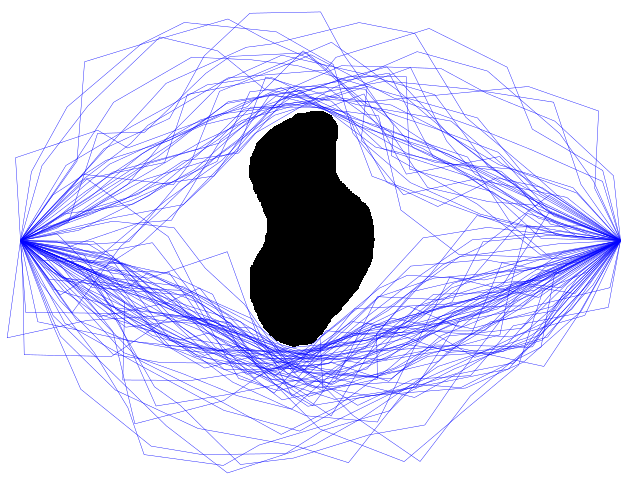
\includegraphics[width=5.5cm]
         {figs/bean/bean-typenopadding-lambda0p0000.png}};
      \node[anchor=south east] at (pic1.south east) {$\lambda = 0$};
      \node[anchor=north] at (pic1.south) {Length: 724.3 \quad Plan Cost: 6740.4};
      \node[inner sep=0pt] (pic1) at (0,-4.7) {
         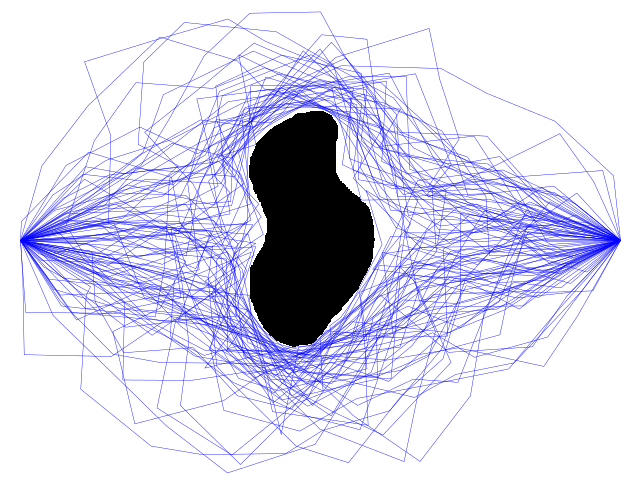
\includegraphics[width=5.5cm]
         {figs/bean/bean-typenopadding-lambda0p9999.png}};
      \node[anchor=south east] at (pic1.south east) {$\lambda = 1$};
      \node[anchor=north] at (pic1.south) {Length: 804.8 \quad Plan Cost: 4540.7};
      \end{tikzpicture}
   }
   % middle
   \subfloat[][%
      \centering
      LEMUR with ``black-box'' broad-phase check
      (not exposed to planner).
      \label{subfig:broad-phase-2d:paddedblackbox}
   ]{
      \begin{tikzpicture}[font=\small]
      \node[inner sep=0pt] (pic1) at (0,0) {
         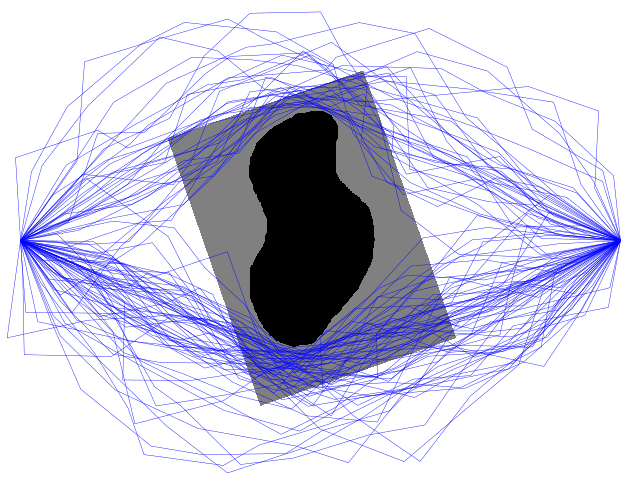
\includegraphics[width=5.5cm]
         {figs/bean/bean-typepaddedblackbox-lambda0p0000.png}};
      \node[anchor=south east] at (pic1.south east) {$\lambda = 0$};
      \node[anchor=north] at (pic1.south) {Length: 724.3 \quad Plan Cost: 2144.7};
      \node[inner sep=0pt] (pic1) at (0,-4.7) {
         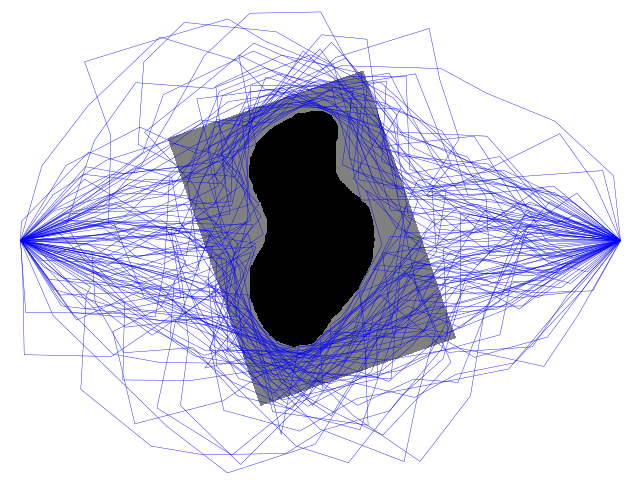
\includegraphics[width=5.5cm]
         {figs/bean/bean-typepaddedblackbox-lambda0p9999.png}};
      \node[anchor=south east] at (pic1.south east) {$\lambda = 1$};
      \node[anchor=north] at (pic1.south) {Length: 804.8 \quad Plan Cost: 1960.6};
      \end{tikzpicture}
   }
   % right
   \subfloat[][%
      \centering
      LEMUR with broad-phase check exposed as a distinct testable subset.
      \label{subfig:broad-phase-2d:paddedutility}
   ]{
      \begin{tikzpicture}[font=\small]
      \node[inner sep=0pt] (pic1) at (0,0) {
         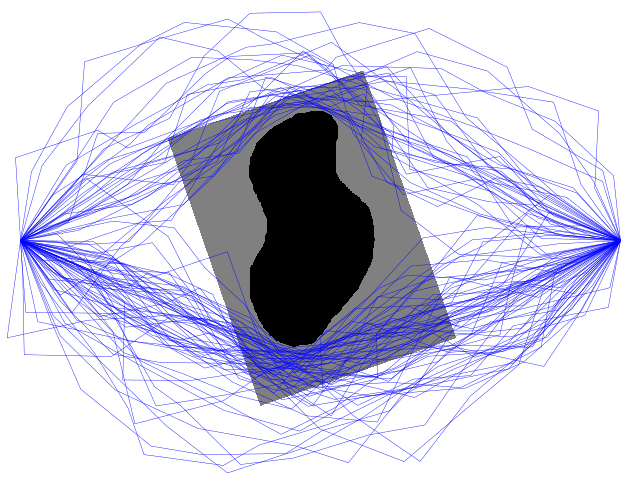
\includegraphics[width=5.5cm]
         {figs/bean/bean-typepaddedutility-lambda0p0000.png}};
      \node[anchor=south east] at (pic1.south east) {$\lambda = 0$};
      \node[anchor=north] at (pic1.south) {Length: 724.3 \quad Plan Cost: 2176.0};
      \node[inner sep=0pt] (pic1) at (0,-4.7) {
         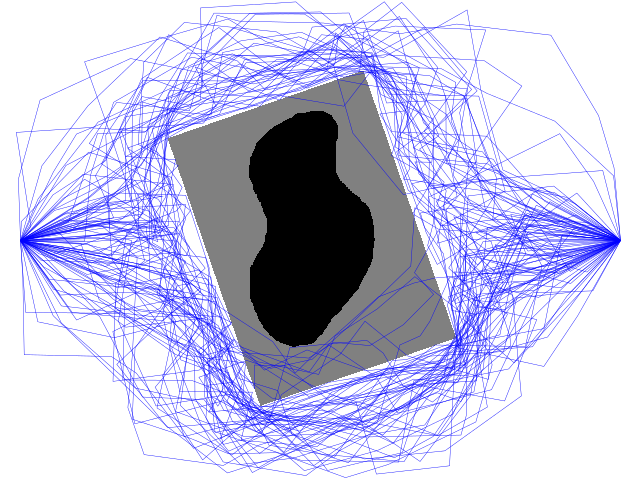
\includegraphics[width=5.5cm]
         {figs/bean/bean-typepaddedutility-lambda0p9999.png}};
      \node[anchor=south east] at (pic1.south east) {$\lambda = 1$};
      \node[anchor=north] at (pic1.south) {Length: 911.4 \quad Plan Cost: 1012.4};
      \end{tikzpicture}
   }

   \caption[][0.5cm]{A simple 2D motion planning example
      in which LEMUR has a broad-phase check available.
      Testing against the bounding box (grey)
      is 10x less expensive than testing
      against the actual obstacle (black).
      Exposing the broad-phase check to LEMUR as a distinct subset
      allows for reduced planning cost.}
   \label{fig:broad-phase-2d}
\end{figure*}

\cdnote{
More caching!
Hypothesized volumes / Cell decompositions.
Bored robots.
Similarity to Leven/Hutchenson.
}

\paragraph{Maximizing Utility in Expectation.}
The strategy of progressively densifying the roadmap discretization
(including the infinite stack approach discussed
in Section~\ref{subsec:conclusion:infinite-stack})
is commonly used for motion planning problems.
Its purpose is to serve as a proxy for handling the spatial coherence
between C-space obstacles in the scene.
For example,
consider motion planning in an environment with many very small
randomly placed obstacles --
in such a scene, it would be difficult to motivate using a coarse
roadmap to confine the search.
What if we handle this more explicitly?

The LEMUR algorithm exploits an optimistic assumption when considering
candidate paths for prospective evaluation:
it assumes all unevaluated edges are collision-free.
While this assumption allows the inner loop to process candidates
quickly,
it requires the hard batching approach to strike an artificial
balance between local and global exploration.
It is worth investigating whether abandoning the optimistic
assumption is worthwhile --
a replacement could then reason explicitly about the collision
probability across the configuration space.

We recently proposed a first step in this direction
via the Pareto Optimal Motion Planner \citep{choudhury2016pomp}.
In this work,
we maintain a probabilistic model of the probability of collision
across the configuration space,
which we update incrementally as collision checks are performed
against the environment.
The planner then uses this model in order to select candidate paths
for partial evaluation that minimize some combination of the path's
execution cost and its probability of collision.
We show that this combination is approximately equivalent
to maximizing utility in expectation
if each colliding path segment is assigned a penalty cost.

%The purpose of the incremental graph densification strategy
%achieved by hard batching (Chapter~\ref{chap:utility})
%is to account for spatial correlation
%in $\mathcal{C}_{\mbox{\scriptsize free}}$.
%We would like to motivate this more formally.
%
%We propose to extend the E$^8$-PRM planner
%to minimize ensemble effort \emph{in expectation}
%using a probabilistic model of $\mathcal{C}_{\mbox{\scriptsize free}}$.
%Even if this is too expensive,
%we can motivate the incremental densification idea,
%with a graduated cost model
%to approximate a probabilistic model
%of the C-space.
%
%How should discrete graphs be constructed in continuous
%   C-spaces with spatially correlated execution costs?
%
%Chapter~\ref{chap:graphs-in-continuous}
%discusses how to embed roadmaps in $\mathcal{C}$
%so that they can be searched by E$^8$.
%
%The problem with na\"{\i}vly running E$^8$ on a
%dense roadmap in $\mathcal{C}$
%is that it tends to bunch up in local minima.
%This is because reducing the continuous planning problem
%to a graph search ignores the spatial correlation
%inherent in $\mathcal{C}_{\mbox{\scriptsize free}}$.
%
%One way to capture this is to maintain a probabilistic model
%of $\mathcal{C}_{\mbox{\scriptsize free}}$,
%and then optimize in expectation.
%In particular,
%instead of greedily choosing the best path based on
%optimistic estimates of one-time planning and execution cost:
%\begin{equation}
%   f(\pi) = \lambda \hat{f}_p(\pi) + (1-\lambda) \hat{f}_x(\pi),
%\end{equation}
%we instead reason over the total \emph{expected} remaining cost:
%\begin{align}
%   f(\pi)
%      &= E \left[ \lambda f_p(\pi) + (1-\lambda) f_x(\pi) \right] \\
%   &= P_{\mbox{\scriptsize free}}(\pi)
%      \left[ \lambda \hat{f}_p(\pi) + (1-\lambda) \hat{f}_x(\pi) \right]
%      + (1-P_{\mbox{\scriptsize free}}(\pi))
%      \left[ \lambda F_p + (1-\lambda) F_x \right]
%\end{align}
%
%Consider the the problem from Figure~\ref{fig:example-in-expectation}.
%There are an infinite number of paths to the goal,
%each consisting of walking along the sidewalk,
%followed by crossing the street perpendicularly at a particular
%position $x$.
%The sidewalk is known to be collision-free,
%whereas each position on the street must be tested for collision
%with obstacles with planning validation cost $\hat{f}_p(\pi)$
%independent of $x$.
%Execution cost $f_x(\pi)$ is given by $|x|+c$.
%
%Suppose we first test walking straight across the street $\pi_0$
%(knowing nothing, this is clearly the optimistically cheapest path)
%and this is deemed in collision.
%Which path should we consider next (e.g $\pi_a$ or $\pi_b$)?
%
%What is our model for $P_{\mbox{\scriptsize free}}(\pi)$?
%Relate to GPs for classification\citep{rasmussen2006gpml}.
%
%We are operating under assumptions:
%\begin{itemize}
%\item Single-shot greedy (won't choose \emph{sets} of paths
%   which minimize remaining effort)
%\item Operates over \emph{paths} instead of configurations
%   or edges (won't probe points, no explicit exploration)
%\end{itemize}
%
%\begin{figure}
%   \begin{center}
%   \includegraphics{build/example-in-expectation}
%   \end{center}
%   \caption{Simple example problem to illustrate optimizing
%      remaining ensemble cost in expectation.}
%   \label{fig:example-in-expectation}
%\end{figure}

\subsection{Tighter Integration with Task Planning}

A motion planner is one component in a larger planning system for
an articulated robot performing real-world tasks.
For example,
we have solved multi-step motion and manipulation planning tasks
using a hierarchical planning architecture for the CHIMP robot
\citep{dellin2014drc}.
LEMUR aims to serve as a performant lower-level geometric motion
planner which is cognizant of both the quality of its solutions
and the planning cost it incurs to find it,
and we have found that LEMUR provides improved performance for
such tasks.

\paragraph{Heuristics for Task and Motion Planners.}
While it can be used effectively in any task planning environment,
there are  opportunities for improved system performance by
integrating the planner more tightly with other system components.
Recent work has married symbolic reasoning with geometric planning
for tasks with multiple subtasks
as multi-modal planning \citep{hauser2010multi},
temporal logic \citep{bhatia2010temporalgoals},
or hierarchical or bridged representations and interfaces
\citep{cambon2009hybrid}, \citep{gravot2005asymov},
\citep{srivastava2014taskmotion}.
In many cases, these task planners can take as input estimates
of solution quality
for prospective geometric groundings of symbolic subtasks.
The utility model over candidate paths maintained by LEMUR could
serve as an effective feedback mechanism for these higher-level
task planners.

\paragraph{Many-to-Many Objectives.}
As a low-level motion planner,
LEMUR has been formulated for solving single-pair
(``one-to-one'') motion planning queries.
This can be trivially extended to address ``one-to-any''
or ``any-to-any'' queries, where the start or goal configurations are
extended to multiple candidates expressed as start or goal regions.
This can be captured naturally in a shortest-path framework by extending
the graph representation with virtual vertices and edges connecting
to all candidates starts and goals.
However, a higher-level multi-step task planner is often incentivized
to explore many candidate intermediate configurations,
and cultivate prospective paths through them.
One method for expressing these ``many-to-many'' queries is by
modifying the objective given to the lower-level motion planner;
we explored the comprehensive multi-root objective
\citep{dellin2015cmr} to that end.
It would be worthwhile to apply this objective to lazy roadmap motion
planners such as LEMUR.

\paragraph{Edge Selectors for Manipulation Graphs.}
We also highlight that task planners can be viewed as searching
the \emph{manipulation graph} \citep{simeon2004manipulation}
for a feasible solution to the task.
Each edge in the manipulation graph comprises a transit or transfer
path
(or, in more general problem domains, other non-prehensile actions).
The computationally intensive part of solving these graphs is
commonly finding feasible geometric groundings for each edge of this
manipulation graph.
We contend that this problem could be solved directly using the LazySP
algorithm (Chapter~\ref{chap:lazysp}.
In this formulation,
each edge of the task graph would itself entail an invocation of LEMUR
-- but each invocation would share the same underlying roadmap
managed as described in Chapter~\ref{chap:family}.
Edge selectors could then be employed to allocate motion planning
resources only on edges in the manipulation graph
most likely to contribute to a short solution to the task.


\section{Lessons Learned}
\label{sec:conclusion:lessons-learned}

%\ssnote{I think the only thing I'd add to the conclusions is a ``Lessons
%learned''. What did you think were hard or easy when you started and
%did they actually turn out that way?}

A number of issues and questions arose during the design and
implementation of the algorithms in this thesis
that may be useful to researchers that may build on this work.

\paragraph{The Importance of Search.}
My initial examination of motion planning begun with a clear
perceived separation between search-based and sampling-based
approaches.
By focusing on roadmap methods,
I envisioned that the question of how to construct roadmaps
over the configuration space would dominate my investigation.
But my exploration of lazy roadmaps resulted in two
personal realizations.
First,
search-based and sampling-based methods are more similar than they are
usually treated
(a connection first identified by LaValle et. al.
\citep{lavalle2004deterministic}).
And second,
the question of how best to search over roadmaps is far from a settled
question.
This motivated by study of both lazy and dynamic search problems,
and lead directly to the development of LazySP and IBiD,
respectively.
Indeed,
the interaction between edge selection and search is rich
with opportunities for future work.

\paragraph{The Importance of Performance Metrics.}
Progress in robotics depends on a delicate interplay between
new research ideas and motivating real-world applications.
While novel ideas can often have a direct benefit on a wide variety
of applications,
the potential for a particular applications or examples
to drive new research is equally powerful.
In particular,
a performance shortfall of an existing algorithm
often serves not only as a motivation for a new idea,
but as a springboard for developing that idea in the first place.
During my thesis,
I found that committing to a set of benchmark problems,
and being guided by rigorous performance metrics such as path
quality and planning time,
allowed me to identify fruitful research areas.
It also lead to many other implementation improvements
-- such as the pre-allocated (or ``baked'') data structures feature
in our implementation of FCL -- which improved performance
across all motion planners in our arsenal.

\paragraph{Fair Comparisons with Non-Determinism.}
If performance metrics are to be trusted,
it is of paramount importance that planner comparisons be fair
and repeatable,
so that only the factor in question
(e.g. the search or sampling strategy) is varied between experiments.
Not only must all outside factors be held constant,
such as collision checker parameters, resolutions, samplers, roadmaps, etc.,
but I found that the most robust way to handle planners which depend
on randomness is to treat the random seed as an additional parameter,
and to commit to ranges of these seeds for testing.
Not only does this allow for a fairer comparison between planners,
but it allows for a direct comparison between revisions of a particular
planner's implementation,
to more easily measure improvement and spot regressions.
In research we often don't have the bandwidth to implement full
unit test coverage, so such ensemble testing must suffice to maintain
the quality of our implementations.

\paragraph{Implementation Details.}
Writing a performant motion planning implementation,
especially one which relies on cached data structures,
requires focus on inner loops, profiling, and iterative development.
Care must be taken so that the roadmap data structure can be loaded
into memory quickly during planner initialization,
and so that the roadmap can be densified efficiently without
reallocating large blocks of the data structure.
The core roadmap generation and search code should be well-tested --
the implementation used in this thesis was developed over several years,
and was used for everything from figure generation to experiments.
I also found it useful to rely on common data formats,
such as GraphML \citep{brandesetal2002graphml},
to allow interoperability with other software packages.

\section{Concluding Remarks}
\label{sec:conclusion:remarks}

This dissertation explores the integration of two ideas
for efficient motion planning
-- \emph{lazy} and \emph{utility-guided} evaluation.
These key ideas are complementary;
while lazy pathfinding serves to decouple the process of
discovering our options from determining their validity,
utility-guided planning gives us the means to select intelligently
between these options for the most promising.

We exploit roadmaps as a way to discretize our continuous planning
problem into a pathfinding problem on a graph.
But importantly, we do not lose sight of our motion planning domain:
evaluating edge weights is expensive.
Not only does this motivate our approach of lazily determining edge
weights,
but it opens the door to intelligent strategies for allocating our
precious planning resources in the right places.
We proposed edge selectors as a mechanism for doing this over the
edges of a graph
(and we have had fruitful discussions with researchers from other
domains such as satellite trajectory planning
which share our problem's cost structure).

While selectors can capture the problem of resource allocation
over the discrete space,
there is also the question of allocating planning resources between
different levels of densification.
LEMUR addresses this question via batching -- switching to a
progressively better discrete approximation to the continuous problem
until a path is found.
However, we discussed ways in Section~\ref{subsec:conclusion:infinite-stack}
to represent this more naturally during the course of the search itself.
This also opens the door to specialized motion planning hardware
(e.g. GPUs and FPGAs) which can maintain roadmaps efficiently
and in parallel (e.g. \citep{murray2016onachip}).

Importantly,
performing lazy search over roadmaps enables the use of grounded
heuristic estimates over concrete prospective motion path segments.
This directly enables our use of utility functions to guide the planner's
evaluation,
which is especially relevant for autonomous robots performing
human-scale tasks
-- performing tasks with and around people requires robots
that are efficient both in computation and in action,
since people are unaccommodating both of long planning pauses
and of wild and inefficient motions.
The expressiveness of our utility function approach,
which can take advantage of any domain-specific planning heuristics
available,
opens the doors to many opportunities for getting better performance
out of autonomous robots performing helpful recurring tasks in our
day-to-day lives.

